\documentclass[border=6pt]{standalone}
\usepackage{tikz,amsmath,amssymb}
\usetikzlibrary{arrows.meta,positioning,calc,fit,backgrounds}
\definecolor{cres}{HTML}{DBEAFE}\definecolor{cresb}{HTML}{1D4ED8}
\definecolor{catt}{HTML}{FDE68A}\definecolor{cattb}{HTML}{B45309}
\definecolor{cconv}{HTML}{E5E7EB}\definecolor{cconvb}{HTML}{374151}
\definecolor{cemb}{HTML}{DCFCE7}\definecolor{cembb}{HTML}{15803D}
\begin{document}\sffamily\scriptsize
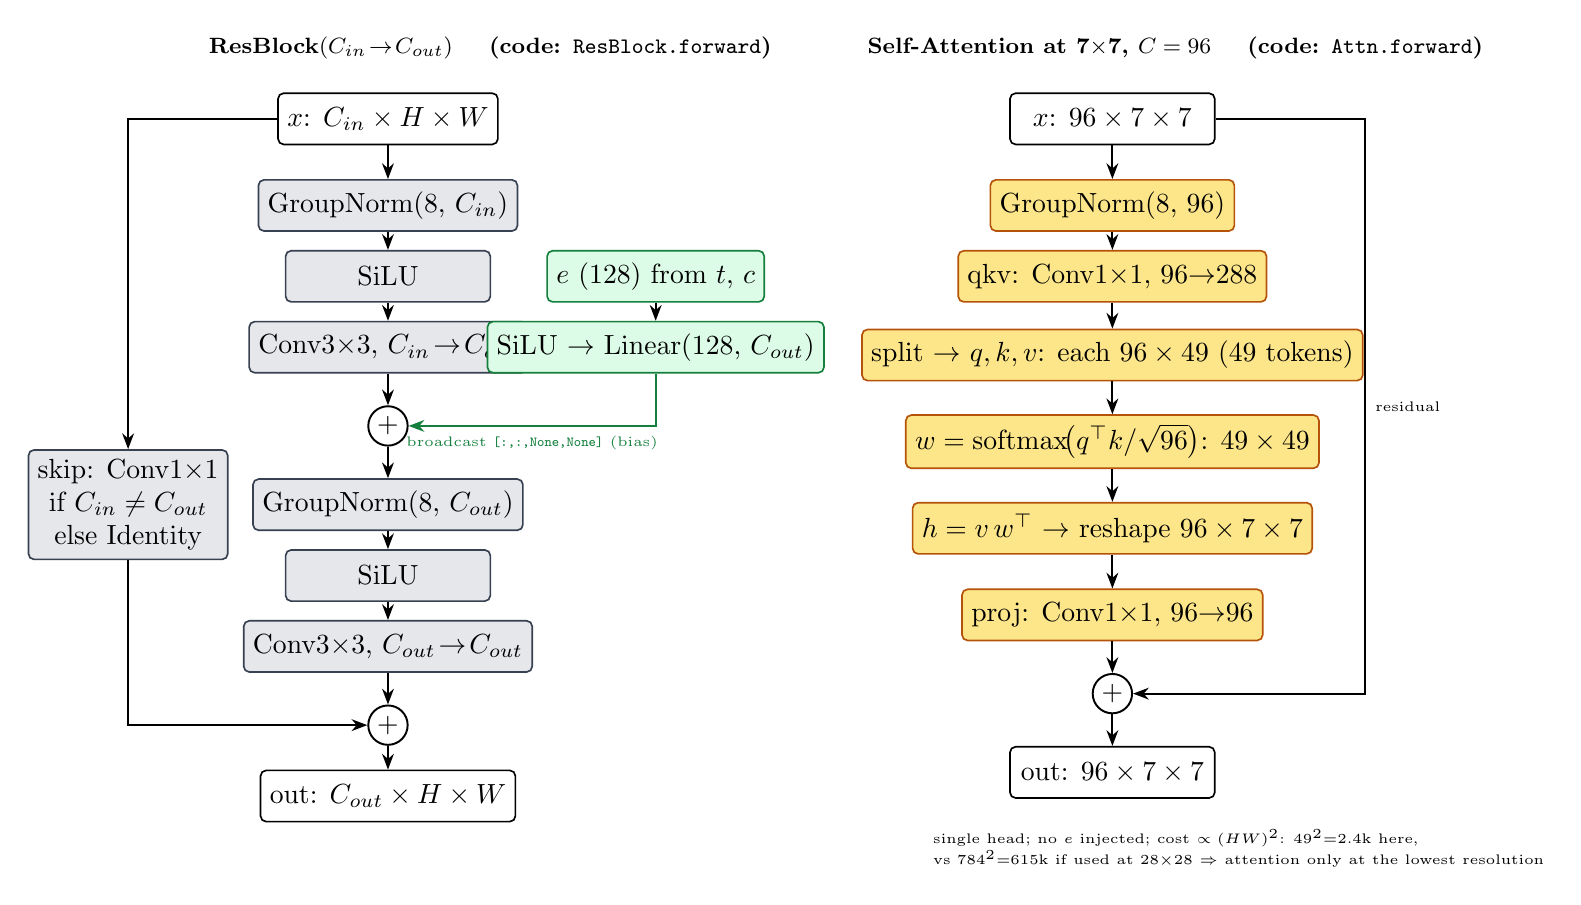
\begin{tikzpicture}[>={Stealth[length=2mm]},
 b/.style={draw,rounded corners=2pt,minimum width=26mm,minimum height=6.5mm,align=center,line width=.6pt},
 n/.style={b,fill=cconv,draw=cconvb}, e/.style={b,fill=cemb,draw=cembb},
 a/.style={b,fill=catt,draw=cattb},
 plus/.style={circle,draw,line width=.7pt,fill=white,inner sep=0pt,minimum size=5mm},
 f/.style={->,line width=.7pt}]
% ===== ResBlock =====
\node[font=\footnotesize\bfseries] at (1.3,0.9) {ResBlock$(C_{in}\!\to\!C_{out})$ \quad (code: \texttt{ResBlock.forward})};
\node[b,fill=white] (x) at (0,0) {$x$: $C_{in}\times H\times W$};
\node[n] (g1) at (0,-1.1) {GroupNorm(8, $C_{in}$)};
\node[n] (s1) at (0,-2.0) {SiLU};
\node[n] (c1) at (0,-2.9) {Conv3$\times$3, $C_{in}\!\to\!C_{out}$};
\node[plus] (p1) at (0,-3.9) {$+$};
\node[e] (ee) at (3.4,-2.0) {$e$ (128) from $t$, $c$};
\node[e] (es) at (3.4,-2.9) {SiLU $\to$ Linear(128, $C_{out}$)};
\node[n] (g2) at (0,-4.9) {GroupNorm(8, $C_{out}$)};
\node[n] (s2) at (0,-5.8) {SiLU};
\node[n] (c2) at (0,-6.7) {Conv3$\times$3, $C_{out}\!\to\!C_{out}$};
\node[plus] (p2) at (0,-7.7) {$+$};
\node[b,fill=white] (y) at (0,-8.6) {out: $C_{out}\times H\times W$};
\node[n,minimum width=22mm] (sk) at (-3.3,-4.9) {skip: Conv1$\times$1\\ if $C_{in}\neq C_{out}$\\ else Identity};
\foreach \u/\v in {x/g1,g1/s1,s1/c1,c1/p1,p1/g2,g2/s2,s2/c2,c2/p2,p2/y,ee/es} \draw[f] (\u)--(\v);
\draw[f,draw=cembb] (es.south) |- node[pos=.75,below,text=cembb,font=\tiny]{broadcast \texttt{[:,:,None,None]} (bias)} (p1.east);
\draw[f] (x.west) -| (sk.north); \draw[f] (sk.south) |- (p2.west);
% ===== Attention =====
\begin{scope}[xshift=9.2cm]
\node[font=\footnotesize\bfseries] at (0.8,0.9) {Self-Attention at 7$\times$7, $C=96$ \quad (code: \texttt{Attn.forward})};
\node[b,fill=white] (ax) at (0,0) {$x$: $96\times7\times7$};
\node[a] (an) at (0,-1.1) {GroupNorm(8, 96)};
\node[a] (aq) at (0,-2.0) {qkv: Conv1$\times$1, 96$\to$288};
\node[a,minimum width=40mm] (sp) at (0,-3.0) {split $\to$ $q,k,v$: each $96\times49$ (49 tokens)};
\node[a,minimum width=40mm] (sm) at (0,-4.1) {$w=\mathrm{softmax}\!\big(q^{\top}k/\sqrt{96}\big)$: $49\times49$};
\node[a,minimum width=40mm] (av) at (0,-5.2) {$h = v\,w^{\top}$ $\to$ reshape $96\times7\times7$};
\node[a] (pr) at (0,-6.3) {proj: Conv1$\times$1, 96$\to$96};
\node[plus] (ap) at (0,-7.3) {$+$};
\node[b,fill=white] (ay) at (0,-8.3) {out: $96\times7\times7$};
\foreach \u/\v in {ax/an,an/aq,aq/sp,sp/sm,sm/av,av/pr,pr/ap,ap/ay} \draw[f] (\u)--(\v);
\draw[f] (ax.east) -- ++(1.9,0) |- node[pos=.25,right,font=\tiny]{residual} (ap.east);
\node[align=left,font=\tiny,anchor=north west] at (-2.4,-8.9) {single head; no $e$ injected; cost $\propto (HW)^2$: 49$^2$=2.4k here,\\ vs 784$^2$=615k if used at 28$\times$28 $\Rightarrow$ attention only at the lowest resolution};
\end{scope}
\end{tikzpicture}
\end{document}
